\section[Relations between \texorpdfstring{$f(t,T)$}{f(t,T)}, \texorpdfstring{$p(t,T)$}{p(t,T)} and \texorpdfstring{$r(t)$}{r(t)}]{Relations between forward rate, zero coupon bond and short rate}
\begin{remark}\lesson{25}{07/05/2020} % Bjork ch. 22.2
    For $S-T=\Delta\to 0$, the LIBOR rate tends to the \emph{spot short rate}, $L(t,t,t+\Delta)$.
\end{remark}
So, we can recover the notion of short rate in terms of LIBOR. We just need a change of notation.
\begin{definition}[Continuously compounded forward rate]
    The continuously compounded forward rate is defined by the equation
    \begin{equation}
        e^{R(t,S,T)(T-S)} = \frac{p(t,S)}{p(t,T)}
    \end{equation}
    from which we get
    \begin{equation}
        R(t,S,T) = \frac{1}{T-S}\ln\left(\frac{p(t,S)}{p(t,T)}\right).
    \end{equation}
\end{definition}
\begin{definition}[Continuously compounded spot rate]
    The continuously compounded spot rate is defined as
    \begin{equation}
        R(S,T) = \frac{1}{T-S}\ln p(S,T).
    \end{equation}
\end{definition}
The continuously compounded spot rate plays the role of the yield in this different notation.
\begin{definition}[Instantaneous forward rate]
    The instantaneous forward rate is defined as
    \begin{equation}\label{forwrate}
        f(t,T) = -\pdv{\ln p(t,T)}{T}
    \end{equation}
\end{definition}
Basically,
\begin{equation}
    f(t,T) = \lim_{\Delta \to 0} (\ln p(t,T) + \ln p(t, T+\Delta))
\end{equation}
In order to well define the relation between the zero coupon bond and the instantaneous forward rate, we can express the price of the zero coupon bond as follows:
\begin{equation}
    p(t,T) = \exp{-\int_t^T f(t,u)\,\dd u}
\end{equation}
Of course, we can introduce also the instantaneous short interest rate.
\begin{definition}[Instantaneous interest rate]
    The instantaneous short interest rate is defined as
    \begin{equation}
        r(t) = f(t,t).
    \end{equation}
\end{definition}
We note that spot rates are forward rates where the time of contracting coincides with the start of the interval over which the interest rate is effective, i.e. $t = S$. The instantaneous forward rate is the limit of the continuously compounded forward rate when $S \to T$. It can thus be interpreted as the riskless rate of interest, contracted at $t$, over the infinitesimal interval $[T,T +\dd T]$.\\
We now go on to define the money account process $B$:
\begin{equation}
    B(t) = e^{\int_0^t} e^{r(s)\,\dd s}
\end{equation}
where $r(s)$ is the instantaneous interest rate. This riskless asset can be seen as the self financing ``rolling-over" trading strategy where for all $t$ we invest in a zero coupon bond starting at time $t$ with maturity $t+\dd t$. In other words, the savings account corresponds to infinite operations of capitalization from time $t$ to time $t+\dd t$ where for each of them we introduce a spot rate $r(s)$ and we immediately reinvest the cash we get. \\
Now, since
\begin{equation}
    p(t,T) = \expect_t\left[e^{-\int_t^T r(s)\,\dd s}\right] = e^{-\int_t^T f(t,u)\,\dd u}
\end{equation}
we are able to link a deterministic expression to a stochastic one. So, the zero coupon bond $p(t,T)$, the short rate $r(t)$ and the forward rate $f(t,T)$ are closely related. This ``static" relationship of couse leads to a ``dynamic" relationship. Therefore, we want to understand which is the relation between $\dd p(t,T)$, $\dd f(t,T)$ and $\dd r(t)$.\\
Let's start from the following general dynamics:
\begin{align}
    \dd r(t) &= a(t)\,\dd t + b(t)\cdot \dd W(t) \\
    \frac{\dd p(t,T)}{p(t,T)} &= m(t,T)\,\dd t + v(t,T)\cdot \dd W(t) \label{zcbdyn} \\
    \dd f(t,T) &= \alpha(t,T)\,\dd t + \sigma(t,T)\cdot \dd W(t) \label{forwratedyn}
\end{align}
where $W(t)$ is the Brownian motion driving the three processes, which can be a vector (we can use the same Brownian motion because all the three processes are responsible for the fluctuations of the interest rate). The only assumptions we make are:
\begin{itemize}
    \item $m, v, \alpha, \sigma \in C^1$ with respect to $T$;
    \item all processes are assumed to be regular enough to allow us to differentiate under the integral sign as well as to interchange the order of integration.
\end{itemize}
Under these regularity assumptions we have the following result.
\begin{theorem}
    The following relationships hold:
    \begin{itemize}
        \item If we know the dynamics of $p(t,T)$, then:
        \begin{align}
            \alpha(t,T) &= \pdv{v(t,T)}{T}v(t,T) - \pdv{m(t,T)}{T} \\
            \sigma(t,T) &= -\pdv{v(t,T)}{T}
        \end{align}
        \item If we know the dynamics of $f(t,T)$, then:
        \begin{align}
            a(t) &= \pdv{f(t,T)}{T} + \alpha(t,T) \\
            b(t) &= \sigma(t,t)
        \end{align}
        \item If we know the dynamics of $f(t,T)$, then:
        \begin{align}
            \frac{p(t,T)}{p(t,T)} = \left(r(t) + A(t,T) + \frac{1}{2}\norm{S(t,T)}^2\right)\,\dd t + S(t,T)\cdot \dd W(t)
        \end{align}
        where
        \begin{align}
            A(t,T) &= -\int_t^T \alpha(t,s)\,\dd s \\
            S(t,T) &= -\int_t^T \sigma(t,s)\,\dd s.
        \end{align}
    \end{itemize}
\end{theorem}
\begin{proof}
    1. From eqs. \eqref{zcbdyn} and \eqref{forwrate}, by applying the Itô formula we have that
    \begin{align*}
        \dd f(t,T) &= - \pdv{(\dd\ln p(t,T))}{T}\\
        &=
        - \pdv{}{T} \left(\left(m(t,T) - \frac{1}{2}v^2(t,T)\right)\dd t + v(t,T)\cdot\dd W(t)\right) \\
        &=
        \left(- \pdv{m(t,T)}{T} + \pdv{v(t,T)}{T}\cdot v(t,T)\right)\dd t - \pdv{v(t,T)}{T}\,\dd W(t)
    \end{align*} % fine parte 1
    2. By integrating the forward rate dynamics \eqref{forwratedyn} we get
    \begin{equation*}\label{pr2}
        f(t,T) - f(0,T) = r(t) - f(0,t) = \int_0^t \alpha(s,T)\,\dd s + \int_0^t \sigma(s,T)\,\dd W(s) \tag{$\star$}
    \end{equation*}
    Now we can write
    \begin{align*}
        \alpha(s,t) &= \alpha(s,s) + \int_s^t \pdv{\alpha}{T}(s,u)\,\dd u \\
        \alpha(s,t) &= \alpha(s,s) + \int_s^t \pdv{\sigma}{T}(s,u)\,\dd u
    \end{align*}
    and taking $t=T$ we can insert this into \eqref{pr2}, getting
    \begin{align*}\label{pr21}
        \notag r(t) - f(0,t) &= \int_0^t \alpha(s,s)\,\dd s + \int_0^t \int_s^t \pdv{\alpha}{T}(s,u)\,\dd u\,\dd s + \\
        &\qquad
        + \int_0^t \sigma(s,s)\,\dd W(s) + \int_0^t \int_s^t \pdv{\sigma}{T}(s,u)\,\dd u\,\dd s \tag{$\ast$}
    \end{align*}
    Using stochastic Fubini in order to change the order of integration we obtain
    \begin{align*}
        r(t) &= f(0,t) + \int_0^t \alpha(s,s)\,\dd s + \int_0^t \,\dd u \int_0^u \pdv{\alpha}{T}(s,u)\,\dd s + \\
        &\qquad
        + \int_0^t \sigma(s,s)\,\dd W(s) + \int_0^t \,\dd u \int_0^u \pdv{\sigma}{T}(s,u)\,\dd s
    \end{align*}
    Now, using Itô we can take the differential:
    \begin{align*}\label{pr22}
        \notag \dd r(t) &= \hlc{mypink}{\pdv{f(s,t)}{T}\,\dd t} + \alpha(t,t)\,\dd t\, \hlc{mypink}{+ \left(\int_0^t \pdv{\alpha}{T}(s,t)\,\dd s\right)\dd t} + \\
        &\qquad
        + \sigma(t,t)\,\dd W(t)\, \hlc{mypink}{+ \left(\int_0^t \pdv{\sigma}{T}(s,t)\,\dd W(s)\right)\dd t} \tag{$\diamond$}
    \end{align*}
    From eq. \eqref{pr21} we have that
    \begin{align*}
        \pdv{f(t,t)}{T} = \pdv{f(0,t)}{T} + \int_0^t \pdv{\alpha(s,t)}{T}\,\dd s + \int_0^t \pdv{\sigma(s,t)}{T}\,\dd W(s)
    \end{align*}
    which is exactly the highlighted term in eq. \eqref{pr22}. So, we obtain the result:
    \begin{align*}
        \dd r(t) = \left(\pdv{f(t,t)}{T} + \alpha(t,t)\right)\dd t + \sigma(t,t)\,\dd W(t)
    \end{align*}
    This is called \emph{Musiela parametrization} and allows to switch from forward rates to short rates. This relation is not immediate, of couse, because the relationship between zero coupon bond price and forward rate is deterministic, but the one between zero coupon bond price and short rate is stochastic.\\
    3. The relationship between the zero coupon price and the forward rate is deterministic:
    \begin{align*}
        p(t,T) = e^{\int_t^T f(t,s)\,\dd s} \equiv e^{Y(t,T)}
    \end{align*}
    From the Itô formula we then obtain the bond dynamics as
    \begin{align*}
        \frac{\dd p(t,T)}{p(t,T)} = \dd Y(t,T) + \frac{1}{2}\dd \expval{Y(\cdot, T)}_t
    \end{align*}
    where
    \begin{align*}
        \dd Y(t,T) = \dd\left(-\int_t^T f(t,s)\,\dd t\right)
    \end{align*}
    and the problem is that in the integral the $t$-variable occurs in two places: as the lower limit of integration and in the integrand $f(t, s)$. This is a situation that is not covered by the standard Itô formula, but it is easy to guess the answer. The $t$ appearing as the lower limit of integration should give rise to the term $\pdv{}{t}\left(\int_t^T f(t,s)\,\dd s\right)\dd t$ and since the stochastic differential is a linear operation, we should be allowed to move it inside the integral, thus providing us with the term $\int_t^T \dd f(t,s)\,\dd s$. Therefore we arrive at
    \begin{align*}
        \dd Y(t,T) &= \dd\left(-\int_t^T f(t,s)\,\dd t\right) \\
        &=
        -\pdv{}{t}\left(\int_t^T f(\hat{t},s)\,\dd s\right)\dd t - \int_t^T \dd f(t,s)\,\dd s \\ % hat(t) means that t is fixed
        &=
        f(t,t)\,\dd t - \int_t^T (\alpha(t,s)\,\dd t + \sigma(t,s)\,\dd W(t))\dd s \\
        &=
        r(t)\,\dd t - \left(\int_t^T \alpha(t,s)\,\dd s\right)\dd t + \left(\int_t^T \sigma(t,s)\,\dd s\right)\dd W(t)
    \end{align*}
    Now we have to compute the quadratic variation of $Y$:
    \begin{align*}
        \dd\expval{Y(t,T)}_t = \left(\int_t^T \sigma(t,s)\,\dd s\right)^2\dd t
    \end{align*}
    Then
    \begin{align*}
        \frac{\dd p(t,T)}{p(t,T)} &= r(t)\,\dd t + \left(- \int_t^T \alpha(t,s)\,\dd s + \frac{1}{2}\left(\int_t^T \sigma(t,s)\,\dd s\right)^2\right)\dd t + \\
        &\qquad\qquad
        + \left(\int_t^T \sigma(t,s)\,\dd s\right)\dd W(t) \\
        &=
        r(t)\,\dd t + \left(A(t,T) + \frac{1}{2}\norm{S(t,T)}^2\right)\dd t + S(t,T)\dd W(t)
    \end{align*}
    which is the result.
\end{proof}

\section{Linear fixed income products}
Linear fixed income products are interest market's products for which the income is fixed by a certain rate of return, even if we know that the return can vary over time due to the randomness of the interest rate. The basic products that we know are the zero coupon bond and the FRA, which are the building blocks that allow to construct the first non trivial product that we consider: the \emph{fixed coupon bond}. This is a bond which, at some intermediary points in time, will provide predetermined payments (coupons) to the holder of the bond. The formal description is as follows.
\begin{itemize}
    \item Fix a number of dates, i.e. points in time, $T_0, \dots, T_n$. Here $T_0$ is interpreted as the emission date of the bond, whereas $T_1, \dots, T_n$ are the coupon dates.
    \item At time $T_i$, $i = 1,\dots, n$, the owner of the bond receives the deterministic
    coupon $c_i$.
    \item At time $T_n$ the owner receives the face value $K$.
\end{itemize}
We now go on computing the price of this bond. It is obvious that the coupon bond can be replicated by holding a portfolio of zero coupon bonds with maturities $T_i$, $i = 1,\dots, n$. More precisely, we will hold $c_i$ zero coupon bonds with maturity $T_i$, $i = 1,\dots, n-1$, and $K+c_n$ bonds with maturity $T_n$. So, the price $p(t)$ at a time $t < T_1$ of the coupon bond is given by
\begin{equation}
    price_t^{\text{FIX}}(t) = K\cdot p(t,T_n) + \sum_{i=1}^n c_i\cdot p(t,T_i)
\end{equation}
Very often the coupons are determined in terms of return, rather than in monetary (e.g. dollar) terms. The return for the $i$-th coupon is typically quoted as a simple rate acting on the face value $K$, over the period $[T_i-1,T_i]$. Thus, if, for example, the $i$-th coupon has a return equal to $r_i$, and the face value is $K$, this means that
\begin{equation*}
    c_i = r_i(T_i - T_{i-1})K.
\end{equation*}
For a standardized coupon bond, the time intervals will be equally spaced, i.e.
\begin{equation*}
    T_i = T_0 + i\delta,
\end{equation*}
and the coupon rates $r_1,\dots,r_n$ will be equal to a common coupon rate $r$. The
price of such a bond will, for $t \le T_1$, be given by
\begin{equation}
    price_t^{\text{FIX}}(t) = K\left(p(t,T_n) + r\delta\sum_{i=1}^n c_i\cdot p(t,T_i)\right)
\end{equation}

\section{Floating rate bonds}
There are various coupon bonds for which the value of the coupon is not fixed at the time the bond is issued, but rather reset for every coupon period. As an example, we will confine ourselves to discussing one of the simplest floating rate bonds, where the coupon rate $r_i$ is set to the spot LIBOR rate $L(T_i-1,T_i)$. Thus
\begin{equation*}
    c_i = (T_i - T_{i-1})L(T_{i-1}, T_i)K,
\end{equation*}
and we note that $L(T_i-1,T_i)$ is determined already at time $T_i-1$, but that $c_i$ is not delivered until time $T_i$. In other words, we need an information involving the forward LIBOR rate. As a consequence, we have two possibilities to price this contract:
\begin{itemize}
    \item Before the crisis, if we set $T_i-T_{i-1} = \delta$ (coupon dates are equally spaced) and $K=1$ we have
    \begin{equation*}
        c_i = \delta L(T_{i-1},T_i) = \delta\left(\frac{1-p(T_{i-1},T_i)}{\delta p(T_{i-1},T_i)}\right) = \frac{1}{p(T_{i-1},T_i)}-1
    \end{equation*}
    This cash flow is delivered at time $T_i$ but it is already measurable at time $T_{i-1}$ with respect to the filtration $\mathcal{F}_{T_{i-1}}$. Now, if we consider
    \begin{align*}
        price_t(c_i) = \expect_t\left[e^{-\int_t^T r(s)\,\dd s}c_i\right]
    \end{align*}
    and we move to the forward measure $\Qmeas^T$ in order to eliminate the random discounting, we get
    \begin{align*}
        \expect_t\left[e^{-\int_t^T r(s)\,\dd s}c_i\right] &= p(t,T_i)\mathbb{E}_t^{\Qmeas^{T_i}}[c_i] \\
        &=
        p(t,T_i)\mathbb{E}_t^{\Qmeas^{T_i}}\left[\frac{1}{p(T_{i-1},T_i)}-1\right] \\
        &=
        p(t,T_i)\mathbb{E}_t^{\Qmeas^{T_i}}\left[\frac{p(T_i,T_i)}{p(T_{i-1},T_i)}-1\right] \\
        \overset{(a)}&{=}
        p(t,T_i)\left(\frac{p(t,T_i)}{p(t,T_i)}-1\right) \\
        &=
        p(t,T_i)-p(t,T_i)
    \end{align*}
    where in (a) we use the martingality of the first term. Since this is the price of a single $c_i$, the total price will be
    \begin{align}
        price_t^{\text{FLOAT}} = p(t,T_n) + \sum_{i=1}^n p(t,T_i)-p(t,T_i) = p(t,T_0)
    \end{align}
    So at the end we move one unit of the notional backward on time using as discount factor the corresponding $c_i$ (because before the crisis we can discount and capitalize with respect to the LIBOR).
    \begin{center}
        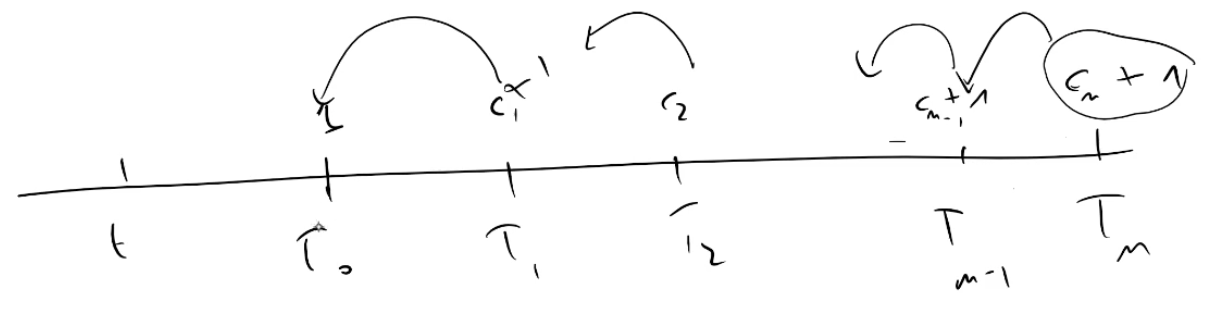
\includegraphics[scale=0.17]{fig/tmp/fig40}
    \end{center}
    In particular, $price_{T_0}^{\text{FLOAT}} = 1$. This means that whatever happens after $T_0$ does not matter because the way in which we pay cash flows is exactly symmetric with respect to the way in which we discount money.
    % continua l'itemize nella lezione successiva
